% Wide figures are declared before the running text so the compositor can fill each page.

\begin{figure*}[!tbp]
\begin{minipage}{\textwidth}
\centering
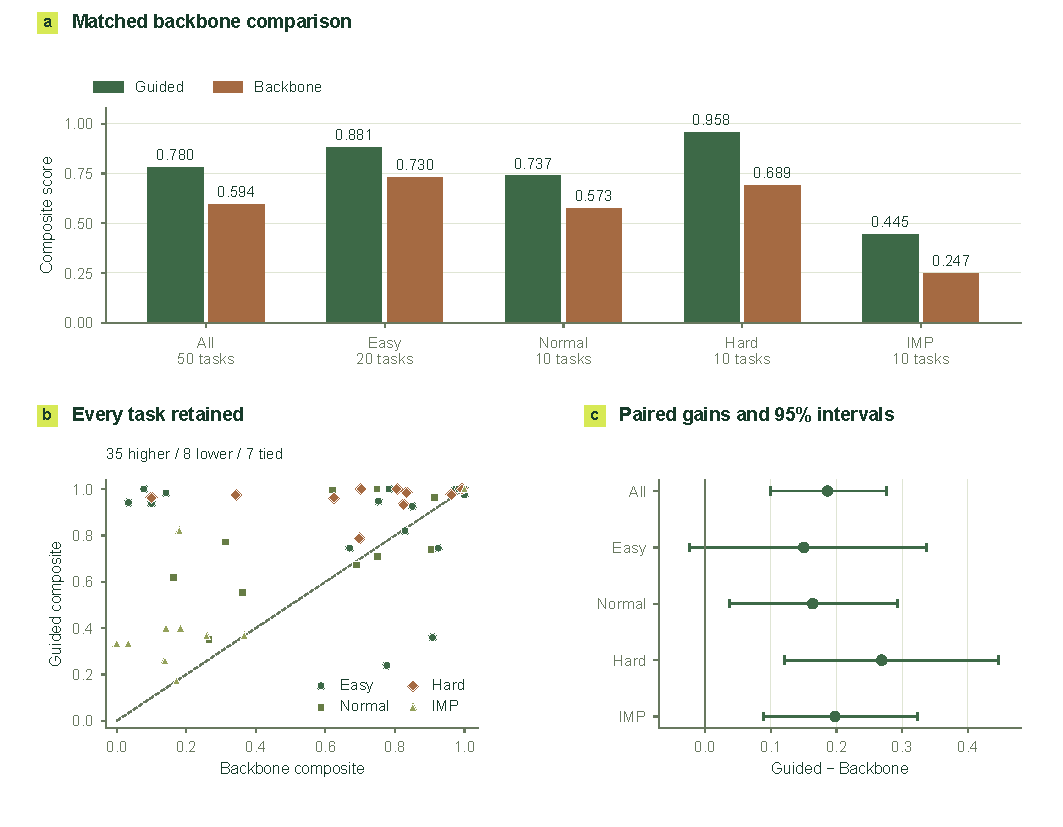
\includegraphics[width=\textwidth]{figures/bench_overview.pdf}
\caption{P2 主比较与逐题差异。a，Cloudra Guided 与同一 backbone 的 Standard 基线在全部 50 题及各难度层的整理后复合分；Easy 为 20 题，其余各 10 题。b，保留全部 50 个同题配对。c，配对均差与 100,000 次按任务整组 bootstrap 的 95\% 百分位区间。}
\label{fig:bench-overview}
\end{minipage}
\end{figure*}

\begin{figure*}[!tbp]
\begin{minipage}{\textwidth}
\centering
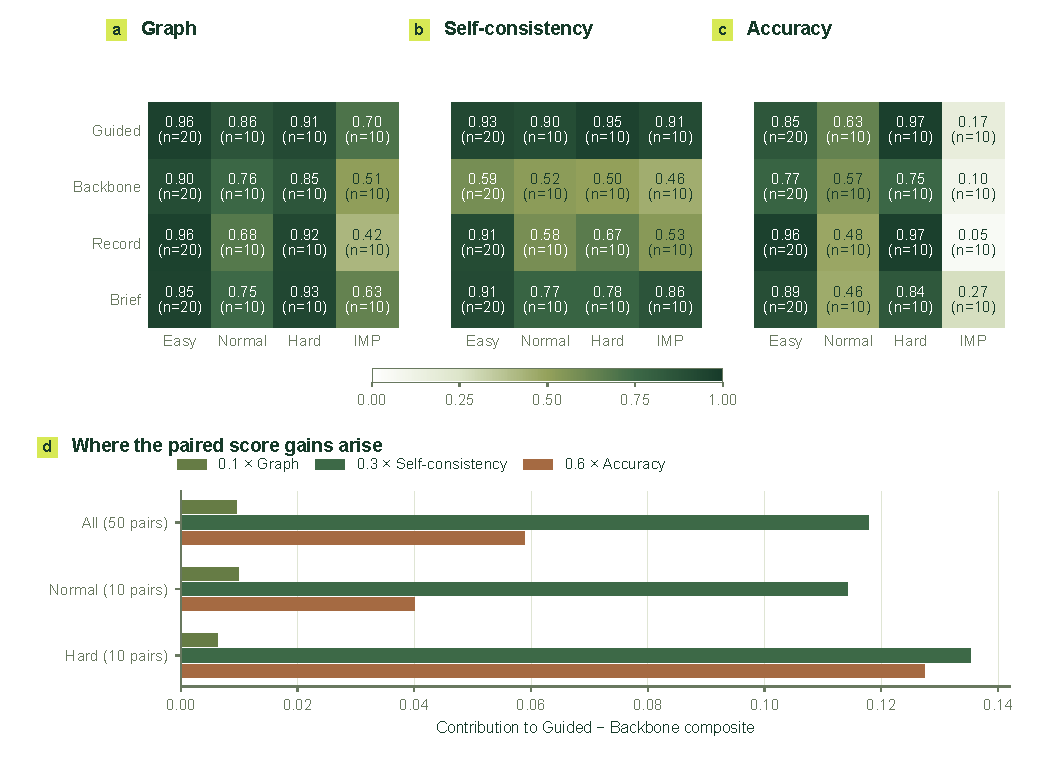
\includegraphics[width=\textwidth]{figures/bench_components.pdf}
\caption{全部200次整理后运行的三个评分层。a--c，各配置、难度层的Graph、自洽性与Accuracy均值；每配置总体50题，Easy为20题，其余各层10题。d，按固定0.1/0.3/0.6权重分解Guided相对Backbone的均差，全部、Normal与Hard分别使用完整50、10和10个配对。各运行分量由其自身研究材料与评分记录对齐至最终整理总分。}
\label{fig:bench-components}
\end{minipage}
\end{figure*}

\begin{figure*}[!tbp]
\begin{minipage}{\textwidth}
\centering
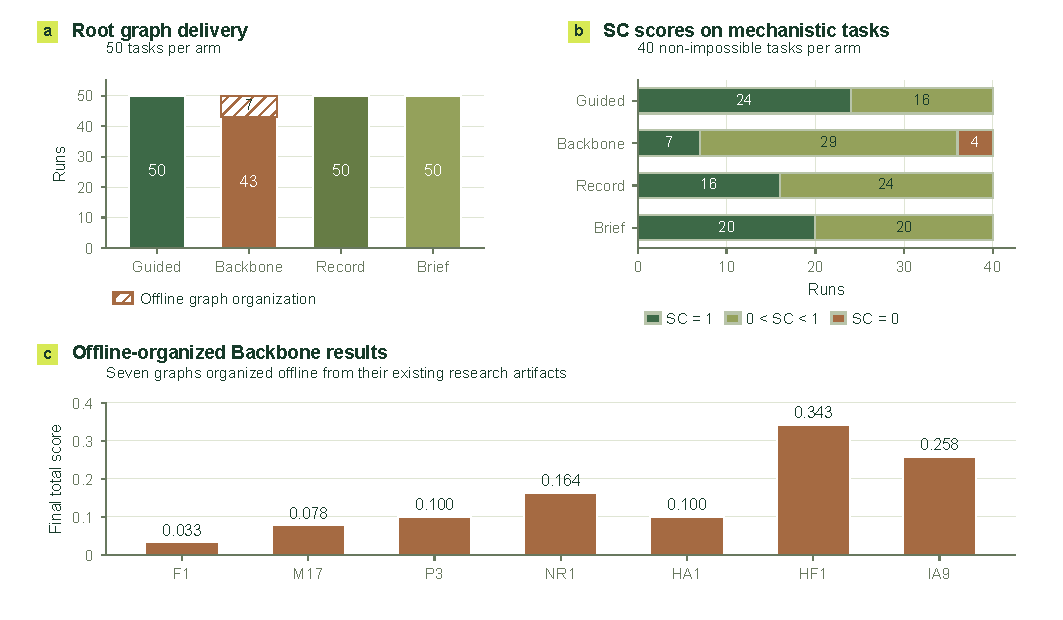
\includegraphics[width=\textwidth]{figures/bench_delivery.pdf}
\caption{运行期交付图与最终科学支持。a，每配置50题中的原始根图记录，Guided、Backbone、Record与Brief分别为50、43、50和50；斜线标记从运行自身材料离线组装的7份Backbone图，整理后每配置均为50份。b，每配置全部40道非Impossible题的自洽分布，区分SC=1、部分正分及SC=0；满分数依次为24、7、16和20，Backbone另有4题零分。c，7个未在运行中形成根图的Backbone任务整理后总分，范围0.0333至0.3425，均值0.1537。}
\label{fig:bench-delivery}
\end{minipage}
\end{figure*}

\begin{figure*}[!tbp]
\begin{minipage}{\textwidth}
\centering
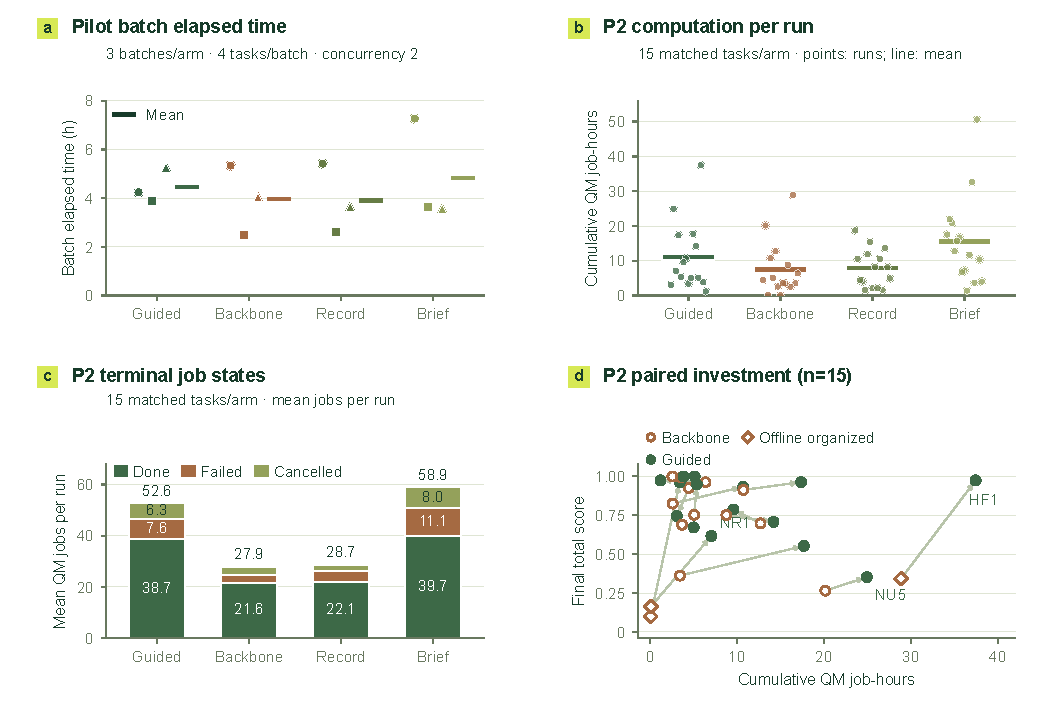
\includegraphics[width=\textwidth]{figures/bench_speed.pdf}
\caption{运行速度与计算投入。a，P1b 的 12 个真实批次，每配置 3 批，每批 4 题，并发为 2；点为观测批次，短线为均值。b，P2 四配置共同 15 题的逐运行累计 QM job-hours 及均值。c，同一任务集每运行的完成、失败和取消作业数量。d，Standard 与 Guided 同题的计算投入及整理后总分，箭头连接相同任务，菱形标记离线组装机理图的运行。}
\label{fig:bench-speed}
\end{minipage}
\end{figure*}

\begin{figure*}[p]
\begin{minipage}{\textwidth}
\centering
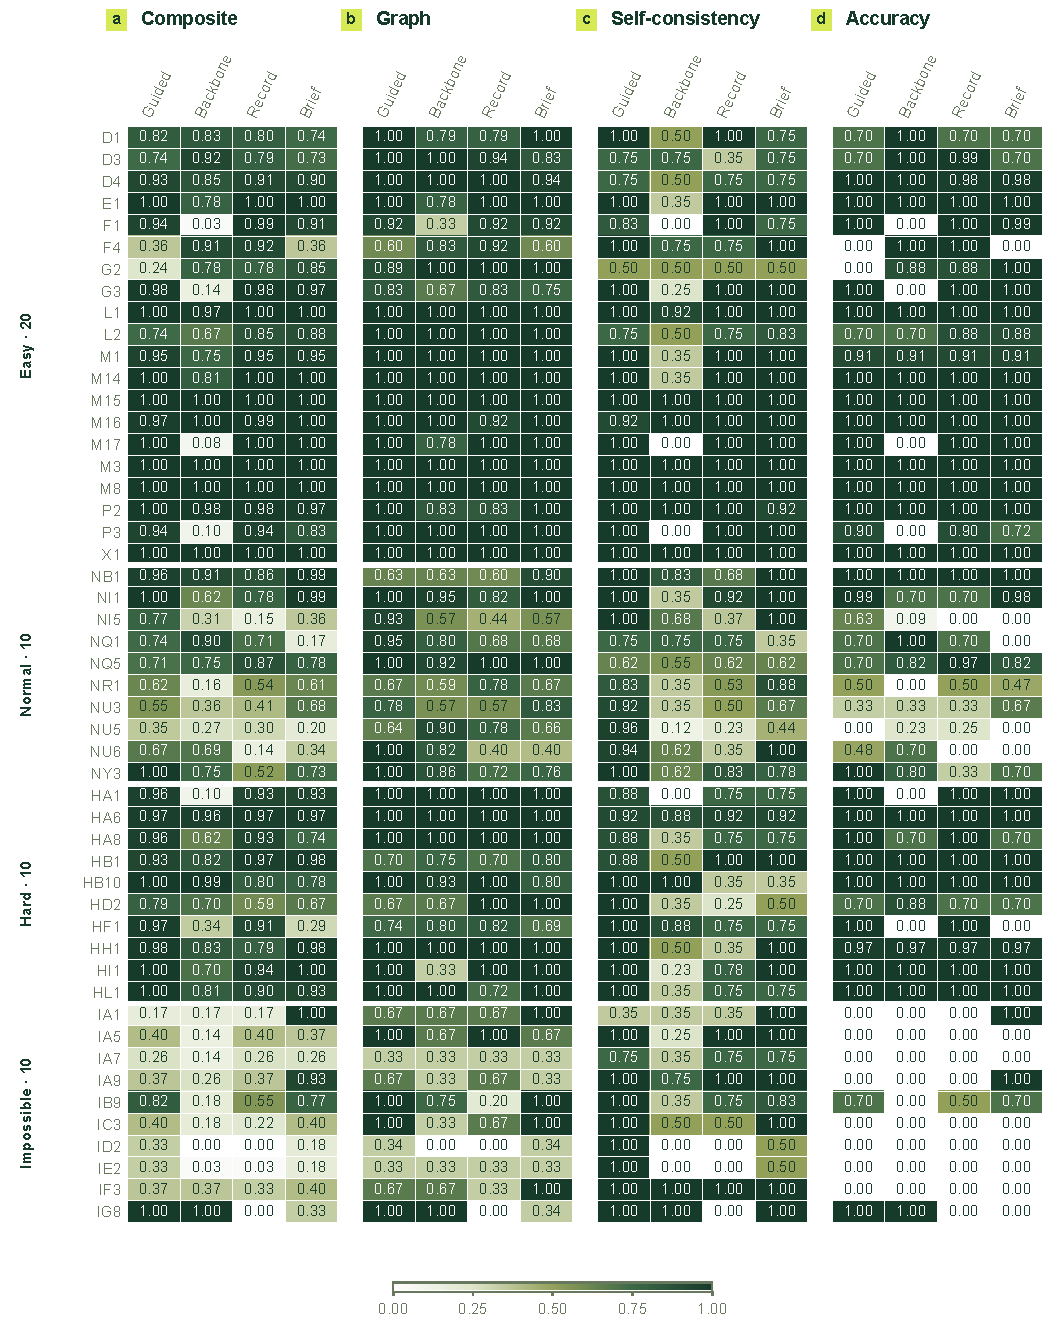
\includegraphics[width=\textwidth]{figures/bench_tasks_all.pdf}
\caption{CloudraBench全部50题、四配置的完整逐题成绩。四个评分块按相同顺序展示综合分、Graph、自洽性与Accuracy，色标统一为0--1，800格全部呈现。数值保留两位小数，来源表保留完整精度。}
\label{fig:bench-tasks}
\vspace{6pt}
\end{minipage}
\end{figure*}

\begin{figure*}[!tbp]
\begin{minipage}{\textwidth}
\centering
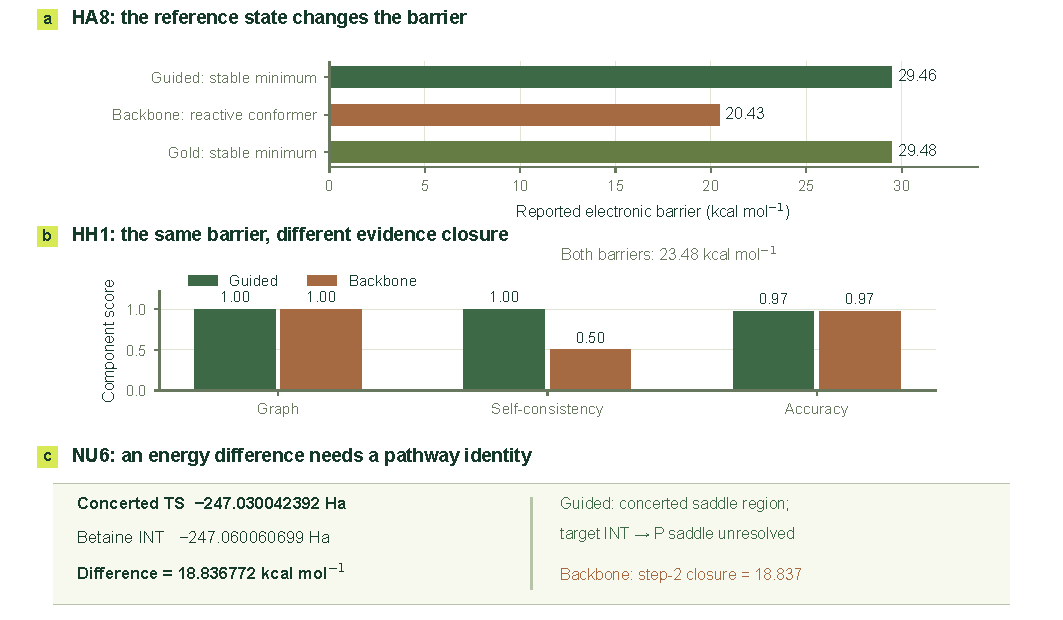
\includegraphics[width=\textwidth]{figures/bench_cases.pdf}
\caption{计算结果的科学归属。a，HA8 分别采用稳定极小值与反应性构象作参照的声明能垒，与 campaign Gold 并列。b，HH1 两组均给出 23.48 kcal/mol 能垒且准确度接近，自洽证据分不同。c，NU6 两个已记录能量之差为 18.836772 kcal/mol；Guided 将其保留为 concerted 鞍点区域的代价，并将目标闭环鞍点留为未解决，Standard 则将 18.837 声明为第二步闭环能垒。计算细节与路径文字取自归档证据记录。}
\label{fig:bench-cases}
\end{minipage}
\end{figure*}

\begin{figure*}[!tbp]
\begin{minipage}{\textwidth}
\centering
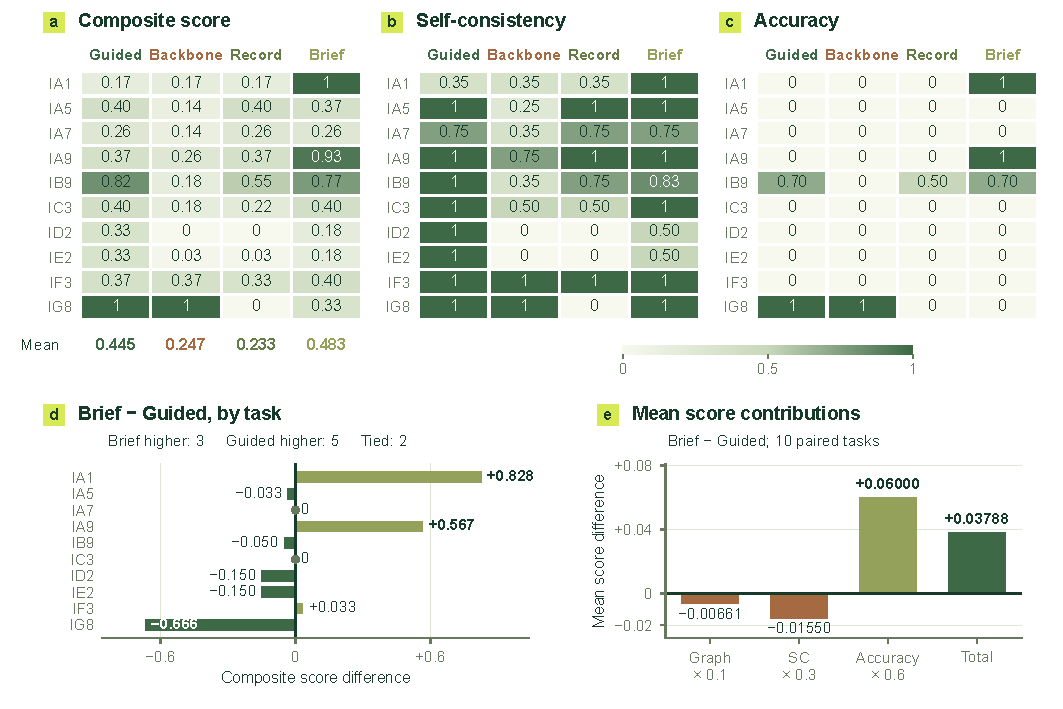
\includegraphics[width=\textwidth]{figures/bench_imp.pdf}
\caption{Impossible层的逐题对照与Brief--Guided差异。a--c，全部10题、四配置的完整整理总分、自洽性和Accuracy，色标统一为0--1。d，Brief相对Guided的逐题总分差，均差+0.03788集中于IA1与IA9，IG8呈相反结果；Guided赢5题、Brief赢3题、2题持平。e，按既定权重分解均差，Accuracy贡献+0.06000、Graph贡献$-0.00661$、自洽性贡献$-0.01550$，细微加总差异来自保存总分的舍入；任务bootstrap的95\%区间为$-0.188$至+0.284，逐题科学声明见下文分析。}
\label{fig:bench-imp}
\end{minipage}
\end{figure*}

\begin{figure*}[!tbp]
\begin{minipage}{\textwidth}

\centering
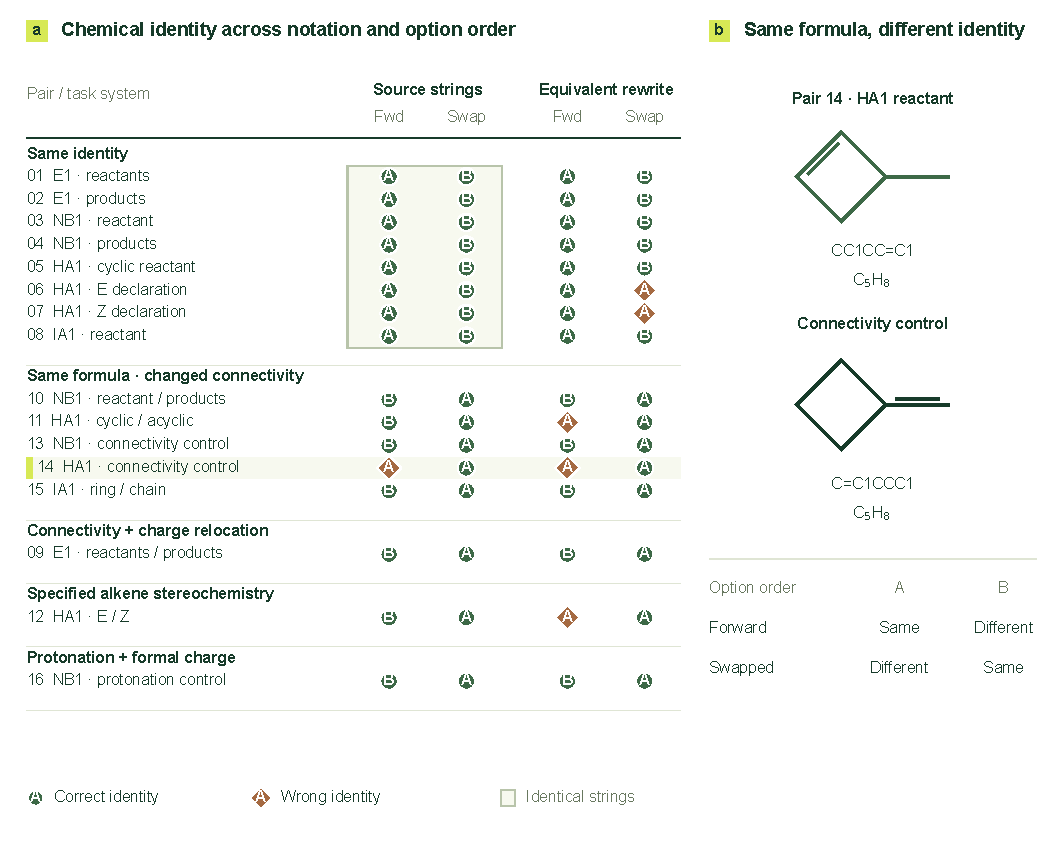
\includegraphics[width=\textwidth]{figures/fig06.pdf}
\caption{分子表示与选项顺序下的化学身份判断。16 对分子各包含四种输入条件；圆形和菱形分别表示正确与错误，内部字母保留模型实际回答。浅色区域为相同字符串条件。右侧显示第 14 对的两种 C\textsubscript{5}H\textsubscript{8} 连接结构及选项含义。 两种连接分别为 \texttt{CC1CC=C1} 与 \texttt{C=C1CCC1}，分子式均为 C\textsubscript{5}H\textsubscript{8}。}
\label{fig:06}
\end{minipage}
\end{figure*}

\begin{figure*}[!tbp]
\begin{minipage}{\textwidth}
\begin{minipage}[t]{.65\textwidth}
\vspace{0pt}
\centering
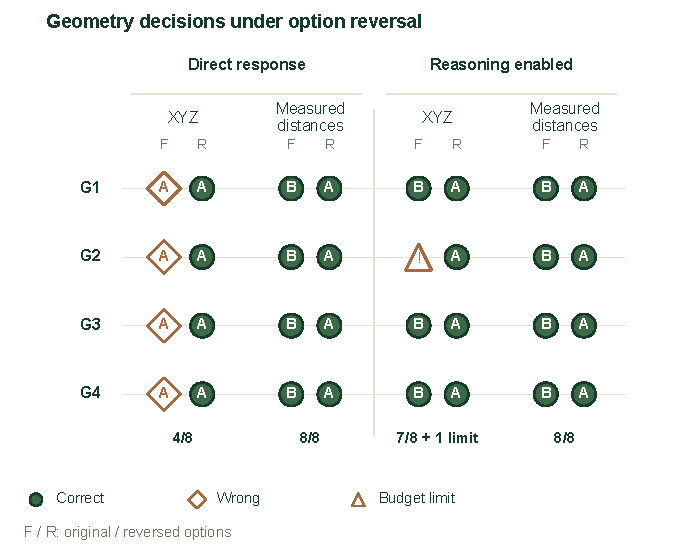
\includegraphics[width=\linewidth]{figures/fig07.pdf}
\caption{坐标输入与测量距离输入下的几何判断。四个源结构分别在直接回答和开启思考条件下比较，每种条件均包含原始（F）与交换（R）选项顺序。圆形表示正确，菱形表示错误，三角形表示达到输出预算；内部字母保留实际回答。}
\label{fig:07}
\end{minipage}\hfill
\begin{minipage}[t]{.31\textwidth}
\vspace{0pt}
\centering
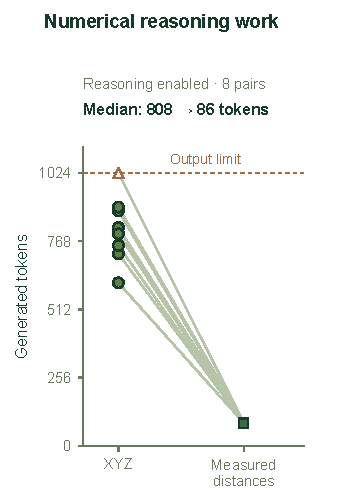
\includegraphics[width=\linewidth]{figures/fig08.pdf}
\caption{开启思考时的生成 token 数。每条线连接同一源结构、同一选项顺序下的笛卡尔坐标输入与测量距离输入，共八组配对比较。虚线表示输出上限。}
\label{fig:08}
\end{minipage}
\end{minipage}
\end{figure*}

\begin{figure*}[!tbp]
\begin{minipage}{\textwidth}
\centering
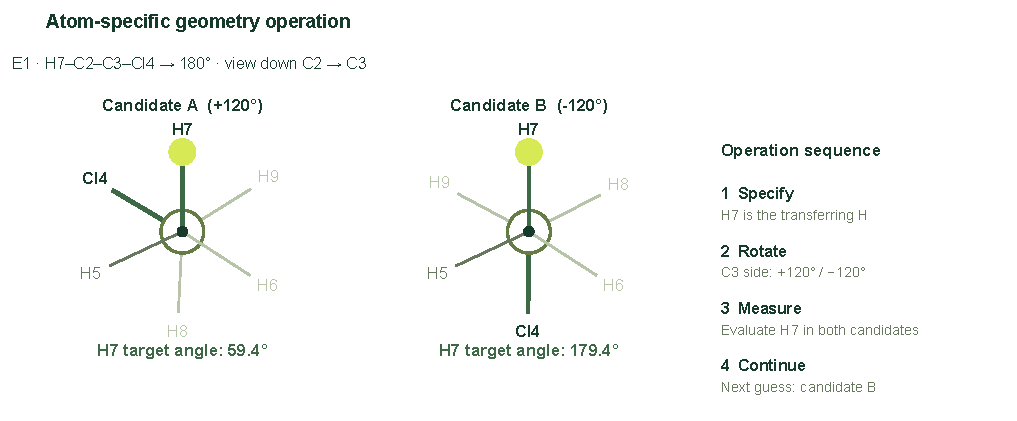
\includegraphics[width=.92\textwidth]{figures/fig09.pdf}
\caption{E1 中面向指定目标的几何操作。Newman 投影保留原候选坐标沿 C2\(\to\)C3 观察时的方向。H7 为指定的转移原子；候选 A、B 的目标角分别为 59.4° 和 179.4°。投影旁列出相应操作顺序。}
\label{fig:09}
\vspace{5pt}
\begin{minipage}[t]{.48\textwidth}
\vspace{0pt}
\centering
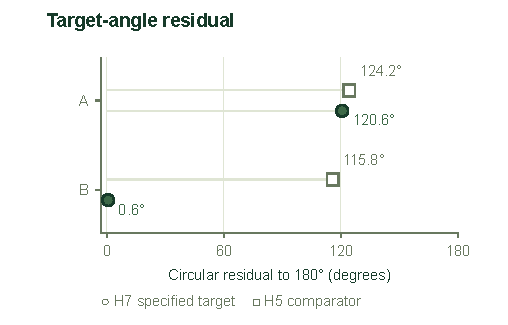
\includegraphics[width=\linewidth]{figures/fig10.pdf}
\caption{候选 A、B 相对指定 180° 目标的圆周角残差。H7 为指定目标原子，H5 为比较原子。}
\label{fig:10}
\end{minipage}\hfill
\begin{minipage}[t]{.48\textwidth}
\vspace{0pt}
\centering
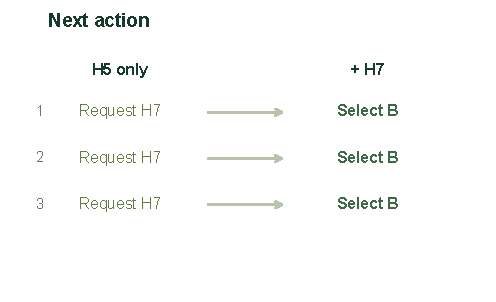
\includegraphics[width=\linewidth]{figures/fig11.pdf}
\caption{三种局部选项排列下的后续动作。仅提供 H5 测量值时，模型请求 H7 测量；补充 H7 后，模型选择候选 B。}
\label{fig:11}
\end{minipage}
\end{minipage}
\end{figure*}

\begin{figure*}[!tbp]
\begin{minipage}{\textwidth}
\centering
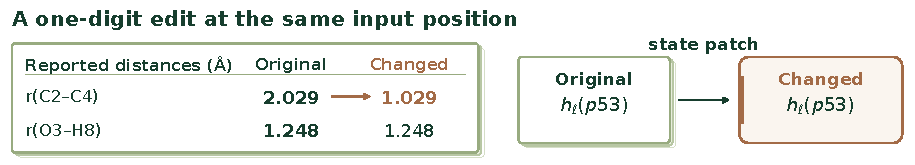
\includegraphics[width=.92\textwidth]{figures/fig12.pdf}
\caption{对单个报告距离的干预。一次数字修改将 C2–C4 距离从 2.029 改为 1.029 Å，O3–H8 保持 1.248 Å。在指定层，将原始输入中 token 位置 53 的残差状态替换到修改后输入的运行中。token 位置从零计数。}
\label{fig:12}
\vspace{4pt}
\centering
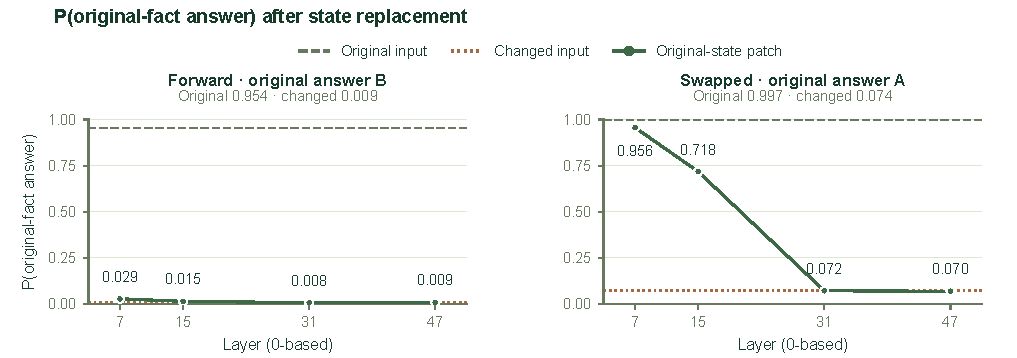
\includegraphics[width=.92\textwidth]{figures/fig13.pdf}
\caption{状态替换后原始事实答案的概率。曲线显示原始顺序（答案 B）与交换顺序（答案 A）下，原始事实答案在完整词表中的概率质量，包含无前导空格与带前导空格的 token 写法。水平线为原始输入与修改后输入的基线。层号从零计数。}
\label{fig:13}
\vspace{4pt}
\centering
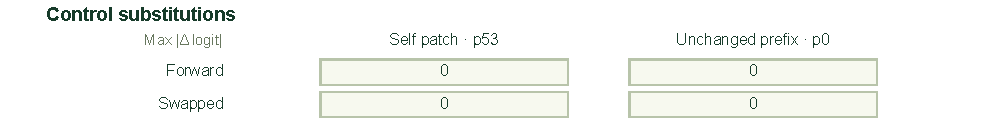
\includegraphics[width=.92\textwidth]{figures/fig14.pdf}
\caption{状态干预实验的对照替换。在 p53 进行同状态自替换，以及在 p0 替换未改变的前缀，两种选项顺序下均保持全部词表 logits 不变。表中报告 logit 差值绝对值的最大值。token 位置从零计数。}
\label{fig:14}
\end{minipage}
\end{figure*}

\begin{figure*}[!tbp]
\begin{minipage}{\textwidth}

\begin{minipage}[t]{.48\textwidth}
\vspace{0pt}
\centering
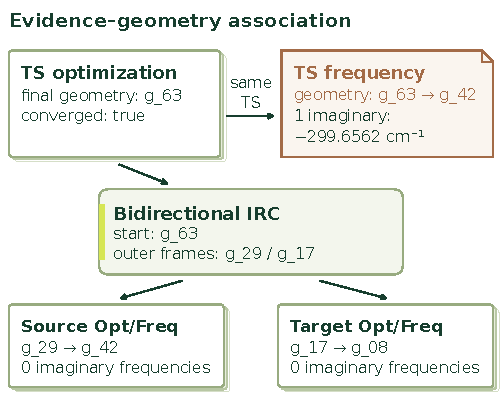
\includegraphics[width=\linewidth]{figures/fig15.pdf}
\caption{E1 源链中的证据与几何关联。受控输入将频率计算的几何引用从 g\_63 改为 g\_42，同时保持局部终止、收敛、能量和频率数值。图中保留从过渡态优化、双向 IRC 到端点优化与频率计算的关联。}
\label{fig:15}
\end{minipage}\hfill
\begin{minipage}[t]{.48\textwidth}
\vspace{0pt}
\centering
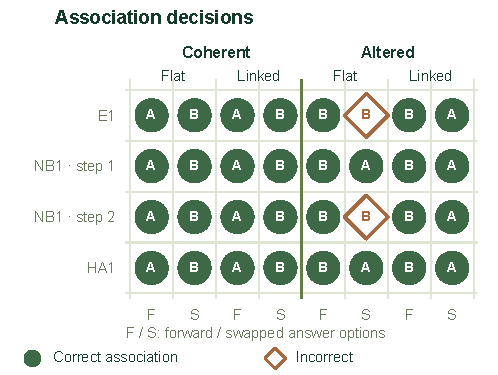
\includegraphics[width=\linewidth]{figures/fig16.pdf}
\caption{四条源链共 32 个输入的关联判断，交叉比较一致或修改后的关联、平铺或关联式表示，以及原始（F）或交换（S）答案顺序。字母保留已保存的 A/B 回答；圆形表示正确关联，菱形表示错误关联。}
\label{fig:16}
\end{minipage}
\end{minipage}
\end{figure*}

\begin{figure*}[!tbp]
\begin{minipage}{\textwidth}
\centering
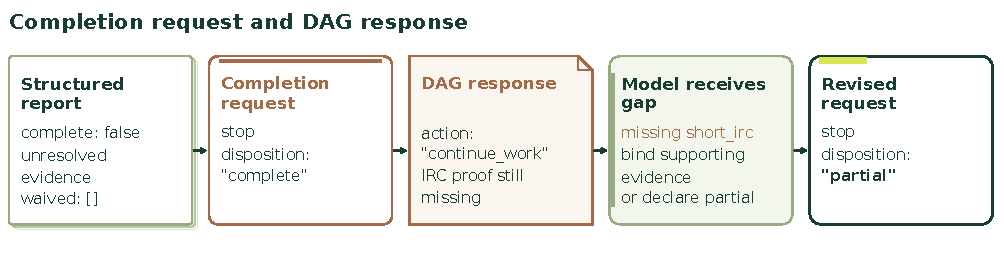
\includegraphics[width=.96\textwidth]{figures/fig17.pdf}
\caption{原始 IA1 轨迹中的完成请求与 DAG 反馈。报告仍有未解决的证据后，模型请求完成；系统指出缺少 short\_irc 证明并向模型反馈，随后模型改为请求部分完成。}
\label{fig:17}
\end{minipage}
\end{figure*}
